\chapter{Introduction}
\label{chap:introduction}

Transport Layer Security (TLS) Protocol is a cryptographic protocol that provides secure transport connection between applications over a computer network, e.g. web server and web browser. 
 Using TLS prevents eavesdropping, tampering and message forgery. It provides privacy and data integrity between communicating applications. The protocol secures transmitted data using encryption. It offers server and, optionally, client authentication to confirm the identities of parties involved in the communication. Further, the integrity check value implemented in the protocol provides integrity of the transfered data. TLS is also known or referred to Secure Socket Layer (SSL), its predecessor. TLS 1.2 was defined in RFC 5246 in August 2008, its successor TLS 1.3 is defined in RFC 8446 in August 2018.
 \cite{RFC5246}

\section{Structure of the TLS Protocol}
\label{sec:stucture}

The TLS Protocol is layered between the Application layer and the TCP/IP layer according to the Internet Model (or between Session and Transport layers according to the OSI Model), where it can secure and then send application data to the transport layer \cite{ms:overview}. Thus it can support multiple application layer protocols, such as HTTP, FTP, SMTP, POP3 and other. The protocols using TLS become respectively HTTPS, FTPS, SMTPS, POP3S and so on.

The TLS Protocol can be split into two layers. The lowest layer of the TLS is the Record Protocol. The upper layer is the Handshake layer, that consists of the following protocols: Handshake Protocol, ChangeCipherSpec Protocol, Alert Protocol. Figure \ref{fig:tls_structure} illustrates the srtucture of the TLS Protocol. 


\begin{figure}[H]
	\centering
		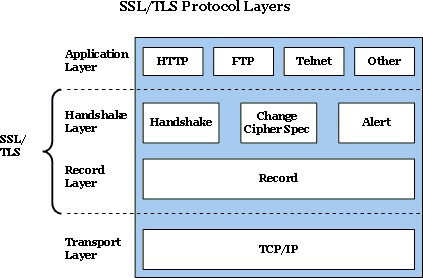
\includegraphics[scale=1]{images/tls_structure.jpg}
	\caption{TLS Protocols Structure \cite{ms:overview}}
	\label{fig:tls_structure}
\end{figure}

\section{Record Protocol}
\label{sec:record_protocol}

The connection with two independent channels is established through the TLS Handshake, from the client to the server and in the other direction from the server to the client. The Record Protocol is responsible for the data protection on these channels using the authenticated encryption scheme.

The processing of data:              
Firstly the Record Protocol layer receives the data from the application layer. Then it fragments the data to a size appropriate to the cryptographic algorithm. 
The next step is compression (optionally, if specified). Then the message authentication code over the compressed data will be computed.
To ensure that the data were not altered during the transmission, the receiver check the incoming MAC value with the computed one if they are matching. Thus the integrity and confidentiality are ensured.
\cite{ms:Record}

\section{Handshake Protocol}
\label{sec:handshake_protocol}
 A handshake is an automated process of negotiation between communicatiors. The TLS Handshake Protocol is the most widely-used  AKE Protocol to negotiate session information between the client and the server. 
 After the etablishment of the TCP connection between a client and a serverer the handshake protocol will trigger. It aims to:  - authenticate the server and eventually the client
 -they also have to agree on the version of the TLS
 -agreement of the ciphersuites
 -arrange the extension
 -derivation authenticated encryption key for the connection
- if required the verifying of the certificates
 After the negotioation the agreements have to be assured.

Due to protecting data these negotiated and defined parameter are then used by the record layer.

\cite{ms:overview}
\cite{ms:handshake}

\section{ChangeCipherSpec Protocol}
\label{sec:changeciphfer_protocol}
This protocol is responsible to change the keys to a new set of keys. 
The keying material is raw data which is used for encryption between the client and server. On the basis of the exchanged information from the handshake protocol, then the keys will be computed.
The ChangeCipherSpec Protocol includes also a message to inform other parties in the SSL/TLS session about the change.   \cite{ms:overview}

The ChangeCipherSpec protocol is removed from the 1.3 version of the TLS protocol.

\section{Alert Protocol}
\label{sec:alert_protocol}
The peer will be noticed by the alert messages about the change in status or error condition (fatal/warning).These messages are also compressed and encrypted. Due to a fatal error the session will close immediately. 

The full list with the alerts, to notify the peer of normal or error condition, is declared in RFC2246 \cite{rfc2246}. \cite{W.Stalling} \cite{ms:overview}

\section{Benefits/Drawbacks, Properties, Characteristic}
\label{sec:introduction_suggestions}



